\chapter{Experimental}

%\emph{\color{gray}Probably need to mention CCD digitaztion pedestal and noise, and dark counts which are zero when cold -- did you do that?.}

This chapter describes the apparatus at Colorado State University which has been used for producing and observing  deposits of Ba/Ba\textsuperscript{+} in SXe.  The main barium source, a Ba\textsuperscript{+} ion beam, is first described, as well as a neutral Ba getter source.  The co-deposit of Ba/Ba\textsuperscript{+} with Xe gas onto a cold sapphire window, subsequent laser excitation, and finally the collection optics for the fluorescence are described.

\section{Ion Beam}

The ion beam system is shown in Fig. \ref{fig:ionbeam}.  This is a clean source of Ba\textsuperscript{+} which can do a very wide range of deposit sizes, from billions of ions in a focused laser region all the way down to the single-ion level and below.
%(may only want to say that if we have those scans)

\begin{figure} %[H]
        \centering
                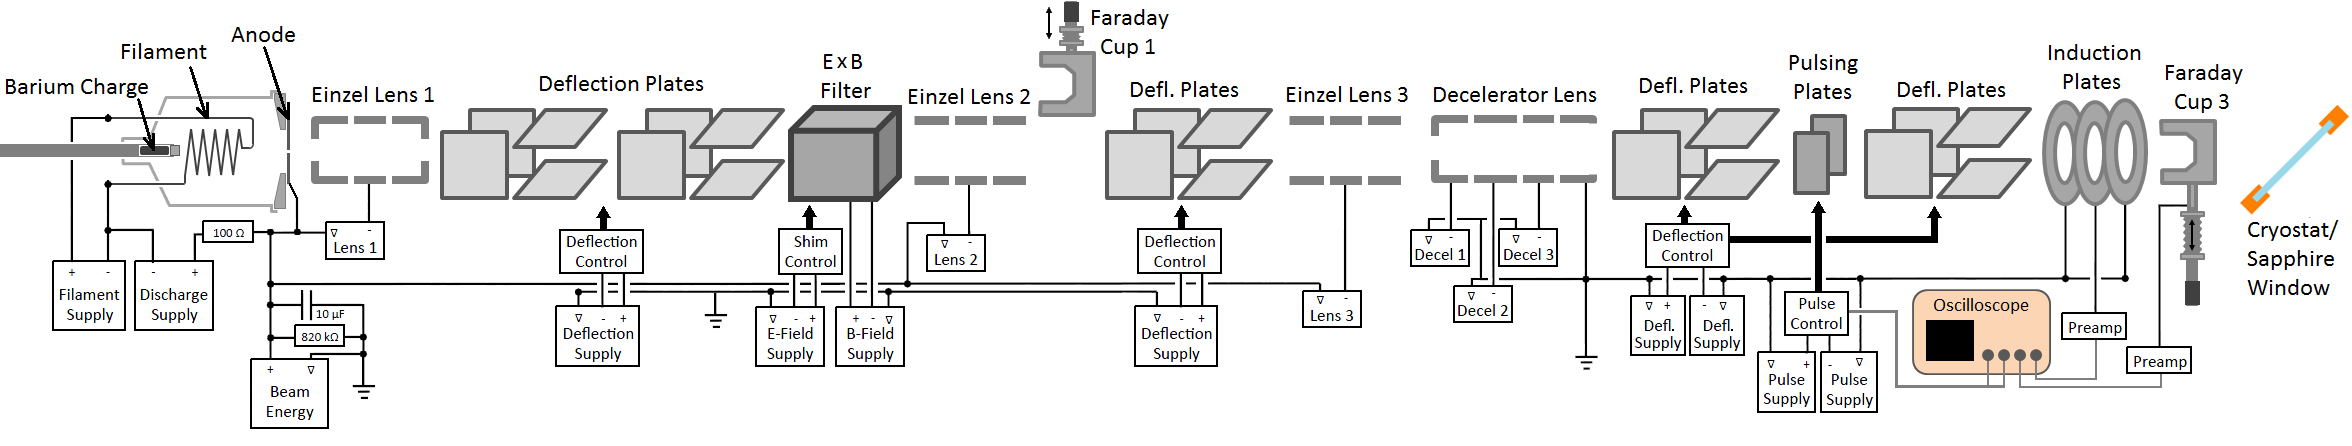
\includegraphics[angle=90,width=.25\textwidth]{figures/ionBeam.png}
                \caption{Ba\textsuperscript{+} ion beam.}
\label{fig:ionbeam}
\end{figure}

\subsection{Ion Source}

Ba\textsuperscript{+} ions are produced in a Model DCIS-101 Colutron ion gun system \cite{Colutron}.  The source is shown in Fig. \ref{fig:ionsource}.  A solid barium charge is placed into the hollowed end of a stainless steel rod, which is inserted into the discharge chamber, where it is heated by a filament.  The barium vaporizes, and escapes the hollowed rod around a loosely threaded set screw.  The source is designed to produce a discharge between the anode plate and the filament cathode, through an argon buffer gas leaked into the source chamber.  This controlled discharge would then also ionize atoms from the solid charge to produce the desired ion beam, and Ar ions would be filtered out.  However, to avoid contamination of the SXe matrix with residual Ar gas, the buffer gas is not used in this work.  We are still able to maintain a discharge with the residual Ba vapor.  The longevity of ion current from a single charge (at least several 10s of hours) suggests that Ba is coating the inner walls of the source chamber, and is heated enough to provide sufficient Ba pressure to support a discharge.  The discharge produces a plasma, containing barium ions, which escapes the chamber through a small hole in the anode, where it enters the acceleration region.  The acceleration potential applied is 2~kV, between the ion source anode and the first element of Einzel lens 1.  This lens approximately collimates the ion beam for passage through the E$\times$B velocity filter.

%This is supported by the observation of white oxidation of the inner source parts after a few minutes of exposure to air when opening the system.

\begin{figure} %[H]
        \centering
                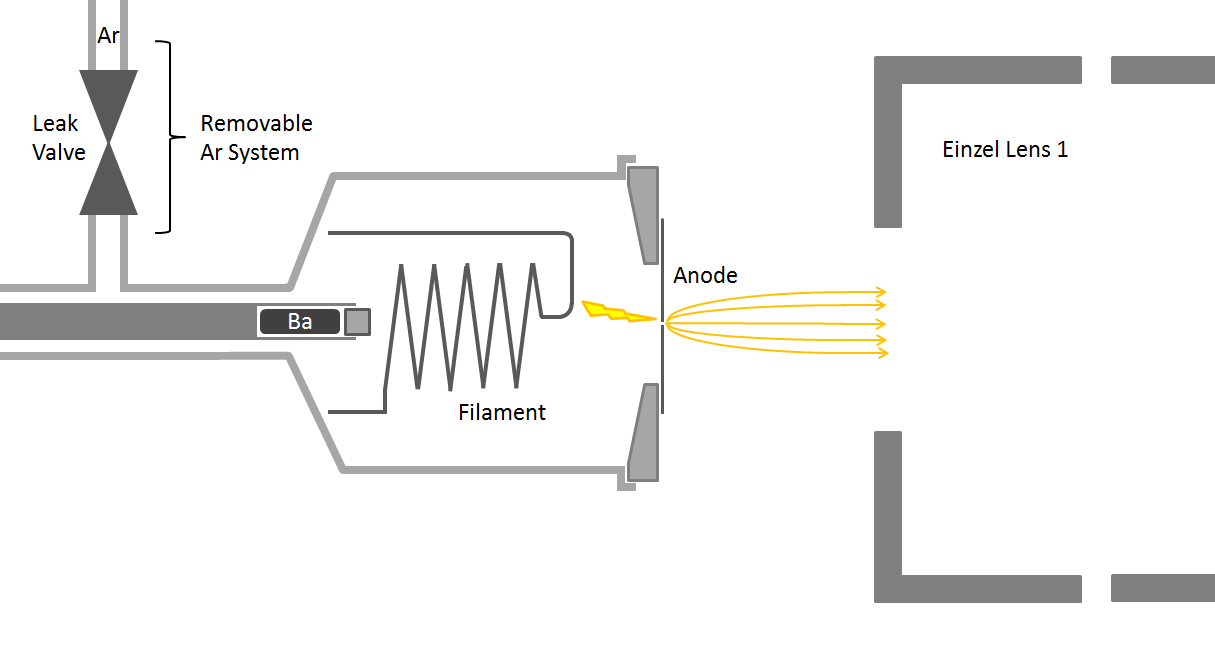
\includegraphics[width=.95\textwidth]{figures/ionSource.png}
                \caption{Ba\textsuperscript{+}/Ar\textsuperscript{+} ion source.}
\label{fig:ionsource}
\end{figure}

\subsection{E$\times$B Velocity Filter}

The E$\times$B velocity filter selects Ba\textsuperscript{+} by creating perpendicular electric and magnetic fields, which produce opposing forces on charged particles moving through the filter.  The opposing forces will be equal for ions with velocity $v = \frac{E}{B}$.  Since ion velocity is determined by mass ($m$), charge ($q$) and beam potential ($V$), the filter selects ions satisfying Eqn. \ref{eqn:massfilt}:

\begin{equation}
\frac{m}{q} = \frac{2 V B^{2}}{E^{2}}
\label{eqn:massfilt}
\end{equation}

\noindent
where $B$ and $E$ are the magnetic and electric fields, respectively.  Those fields are chosen such that Ba\textsuperscript{+} ions pass straight through.  Other ions will be deflected.  

The E$\times$B filter is shown in Fig. \ref{fig:exb}.  Electromagnets provide the vertical magnetic field.  Electrode plates and field-shaping guard rings provide the horizontal electric field.  The guard rings prevent a lensing and astigmatism effect from fringe fields of the plates \cite{Colutron}.

\begin{figure}[h]
        \centering
                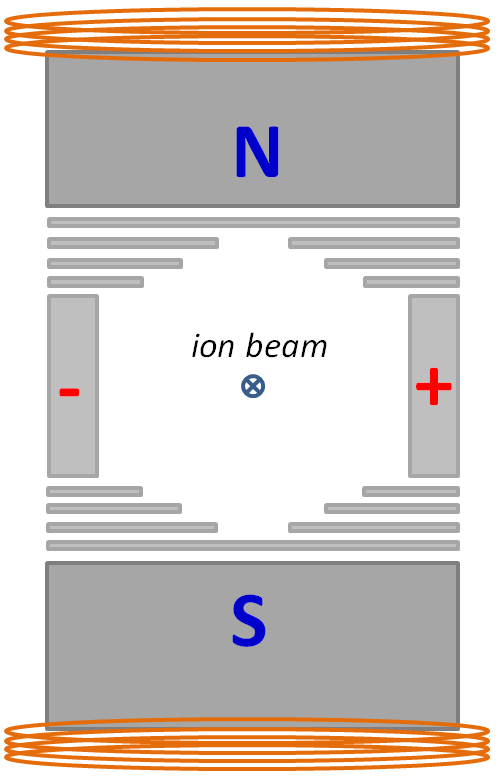
\includegraphics[width=.7\textwidth]{figures/ExB.png}
                \caption{Colutron E$\times$B ion velocity filter.}
\label{fig:exb}
\end{figure}

%\emph{\color{gray}If we need mass scans, we probably need to do new ones with a constant magnetic field, and Ar\textsuperscript{+} and Ba\textsuperscript{+} in same day.  Past scans were all over the place, partly because we were changing beam settings, but new peaks are not very consistent either.}
%To determine the mass components of the beam, the electric field can be scanned.  Mass scans of the Ba\textsuperscript{+} beam is shown in Fig. [ref mass scan fig], as well as of an Ar\textsuperscript{+} beam.  The known mass of Ar aids in calibrating the magnetic field, which differs from the calculation given by Colutron, likely due to hysteresis in the magnet.  \emph{\color{gray}The Ba\textsuperscript{+} peak agrees with the Ba mas s... }

\subsection{Other Beam Components}

The first three sets of deflection plates can be used for beam diagnostics, and are set to 0~V during normal operation.  The deflection plates just before the pulsing plates, H1 and V1, are set to constant values of +50~V and 0~V, respectively, which have been selected such that the beam, in both pulsing and continuous modes, can be deposited at the sapphire window for reasonable settings on the final deflection plates, H2 and V2.  As described in Section \ref{subsec:ionDepCal}, different settings in H2/V2 are required for peak ion current in Faraday cup 3 vs. peak deposit at the window.

Einzel lens 2 focuses the beam to pass through the aperture in the first element of the decelerator lens.  Einzel lens 3 is grounded in this setup.  The decelerator lens can be used to vary Ba\textsuperscript{+} deposit energy, which was done in \cite{Shon}, but it in this work it acts as an Einzel lens with only the second element at voltage.  It focuses the beam near the sample and Faraday cup 3 (there is no Faraday cup 2 in this setup).  Faraday cup 3 measures the ion current during experiments, and is retracted when deposits are being made.  Calibration of deposits using Faraday cup 3 is described in Section \ref{subsec:ionDepCal}.  Faraday cup 1 is used for beam diagnostics, and is usually retracted.  

\emph{\color{gray}on from ion beam studies back when?  At least the procedure for alignment?}

\subsection{Ion Beam Pulsing}

When running in pulsing mode, the pulsing plates are normally set to 200~V and -200~V to deflect the beam, and are pulsed to 0~V for 1~$\mu$s to pass a short pulse of ions straight forward.  The pulsing circuit is shown in Fig. \ref{fig:pulse_circuit}.  Square waves, triggered by LabVIEW at 500~Hz, enter the circuit at (a). The transformed pulse triggers the MOSFET switch, which closes the circuit for the period of the pulse.

\begin{figure} %[h]
        \centering
                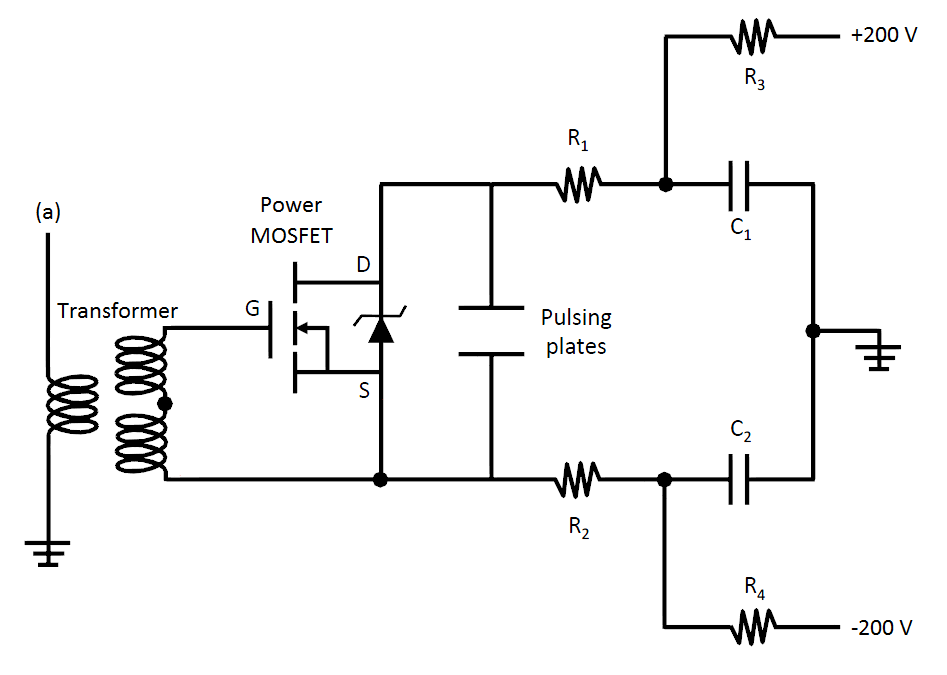
\includegraphics[width=.85\textwidth]{figures/pulsing_circuit.png}
                \caption{Pulsing circuit.  R$_{1}$ = R$_{2}$ = $470~\Omega$, R$_{3}$ = R$_{4}$ = 20~k$\Omega$, \newline C$_{1}$ = C$_{2}$ = 680~nF. \cite{Shon}}
\label{fig:pulse_circuit}
\end{figure}

The induction plates are used to observe pulses during a deposit.  Pulses just prior to a deposit can be observed by cup 3 (as well as the induction plates) for a measurement of ion current in the pulses.  eV Products pre-amplifiers convert the ion current to voltage signals, which are recorded on a digital oscilloscope.  An example of raw oscilloscope traces of Faraday cup 3 and induction plate signals are shown in Fig. \ref{fig:pulse_raw_shaped}(a).  The pre-amp output voltage is related to the input current according to Eqn. \ref{eqn:preamp}:

\begin{equation}
I = \frac{-(V_{out} + R_{1} C \frac{dV_{out}}{dt})}{R_{1} M}
\label{eqn:preamp}
\end{equation}

\noindent
$R_{1} C$ and $R_{1} M$ are determined by putting a known square pulse into the pre-amp.  First, the time constant of an exponential fit to the signal decay determines $R_{1} C$, and then $R_{1} M$ is determined by matching this shaped signal to the original square pulse.  Actual currents in the induction plates and cup 3 are shown in Fig. \ref{fig:pulse_raw_shaped}(b).  The induction signal is positive as ions are approaching the sensitive plate, and an equal but negative signal is seen after the ions pass through.  The Faraday cup stops the ions, so it produces only a positive induction signal as ions approach it.

\begin{figure} %[H]
        %\centering
        %\begin{subfigure}
                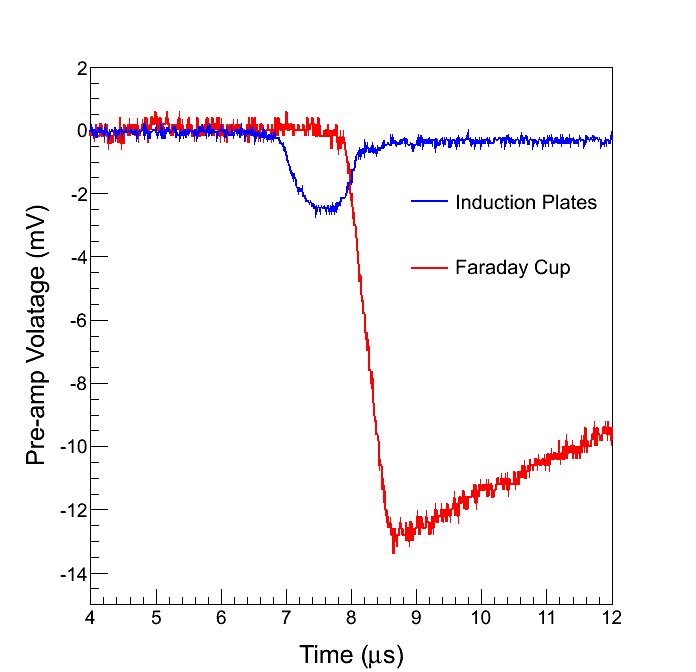
\includegraphics[width=.49\textwidth]{figures/pulse_ind_cup3_raw.png}
                %\caption{barf}
%        %\end{subfigure}
        %\begin{subfigure}
                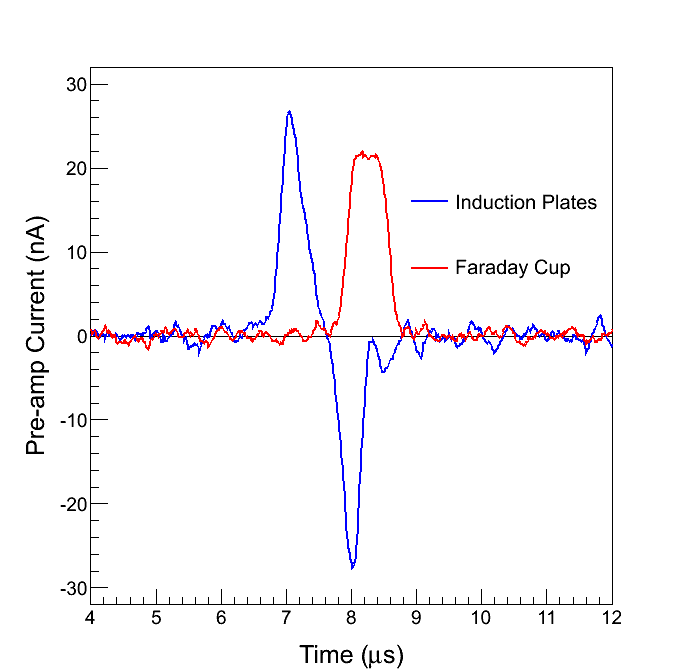
\includegraphics[width=.49\textwidth]{figures/pulse_ind_cup3_shaped.png}
                \caption{Raw (a) and shaped (b) pulse signals from induction plates and cup 3.  The raw induction signal appears small because it is a less sensitive pre-amp (accounted for in shaping).}
        %\end{subfigure}
        \label{fig:pulse_raw_shaped}
\end{figure}

Pulsing data also provides confirmation that the beam is composed of Ba\textsuperscript{+}.  The time between the center of the pulsing plate voltage overlap and the center of the pulse measured by the Faraday cup, along with a measurement of the distance traveled, provides a velocity measurement of the ions.  This distance was measured to be 31.5 $\pm$ 0.5~cm from the center of the pulsing plates to the Faraday cup, and time-of-flight data, e.g. Fig. \ref{fig:pulses_ArBa}, give 39.8 $\pm$ 3.4~amu for Ar\textsuperscript{+} and 136.8 $\pm$ 6.3~amu for Ba\textsuperscript{+}, including an uncertainty on the time of flight of $\pm$ 0.1~$\mu s$.

\begin{figure}[h]
        \centering
                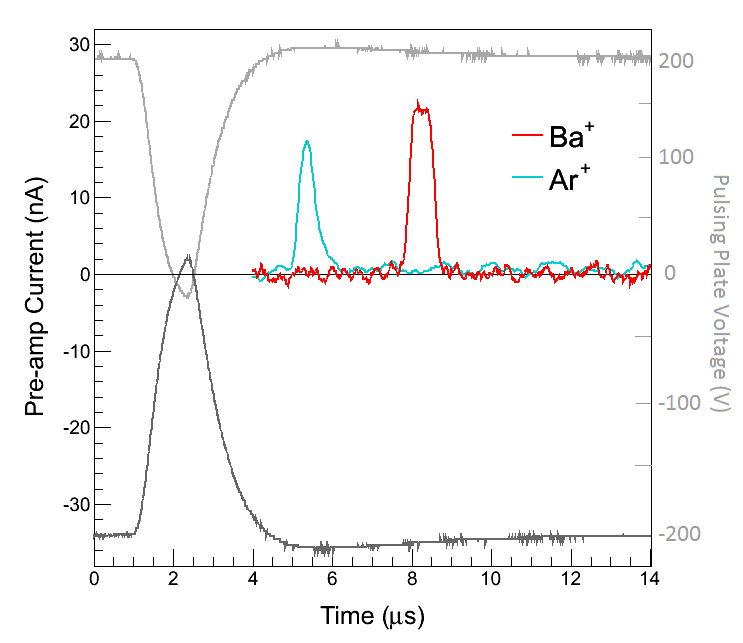
\includegraphics[width=.7\textwidth]{figures/pulses_BaAr.png}
                \caption{Arrival time of pulses at cup 3 vs. time of pulsing plate signal (black (+) and gray (-)) for Ar\textsuperscript{+} and Ba\textsuperscript{+}.}
\label{fig:pulses_ArBa}
\end{figure}

\subsection{Calibration of Ion Deposit}
\label{subsec:ionDepCal}

To calibrate the signal at cup 3 to an ion density at the sapphire window, another Faraday cup (cup W) is attached to the cold finger in place of the sapphire window.  The ratio of $\frac{fC}{pulse}$ between cup 3 and cup W is measured ($\equiv f$).  Then, knowing the radius of the entrance aperture in cup W lets one determine the ion density per pulse at the sapphire window:

\begin{equation}
\frac{ions}{pulse \times m^{2}} = \frac{Q f}{e A}
\label{eqn:ion_density}
\end{equation}

\noindent
where $Q$ is the charge/pulse at cup 3, $A$ is the area of cup W, and $e$ is the elementary charge.  The voltages on the final deflection plates H2 and V2 are also determined to optimize the signal in cup W.  In later experiments, these differed from the values for maximum cup 3 signal by about 70~V in H2 and 60~V in V2, corresponding to about 4~mm in x and y position at cup W, indicating that some drift in optimal ion beam component settings occurred over time, either due to power supply drift or changes in the location of discharge in the source.

\section{Ba Getter Source}

A BaAl$_{4}$ getter, manufactured by SAES, can be inserted on a bellows to emit toward the sapphire window, shown in Fig. \ref{fig:endOfBeamBa}.  When heated, the getter emits neutral Ba with minimal Ba\textsuperscript{+}.  Getters were used extensively in previous work \cite{Brian} for measuring the absorption of Ba in SXe with large Ba deposits, and in identifying emission peaks.  A getter was used briefly in this work in identifying the 619-nm fluorescence peak, as described in Section \ref{sec:619identification}.  The barium getters used in \cite{Brian} were exothermic BaAl$_{4}$-Ni flash getters.  The getter used here is an endothermic BaAl$_{4}$ type, designed for more controlled Ba emission.  

%no evidence is provided in Brian's thesis, nor Shon's, and I don't see anything on the SAES website

\begin{figure} %[h]
        \centering
                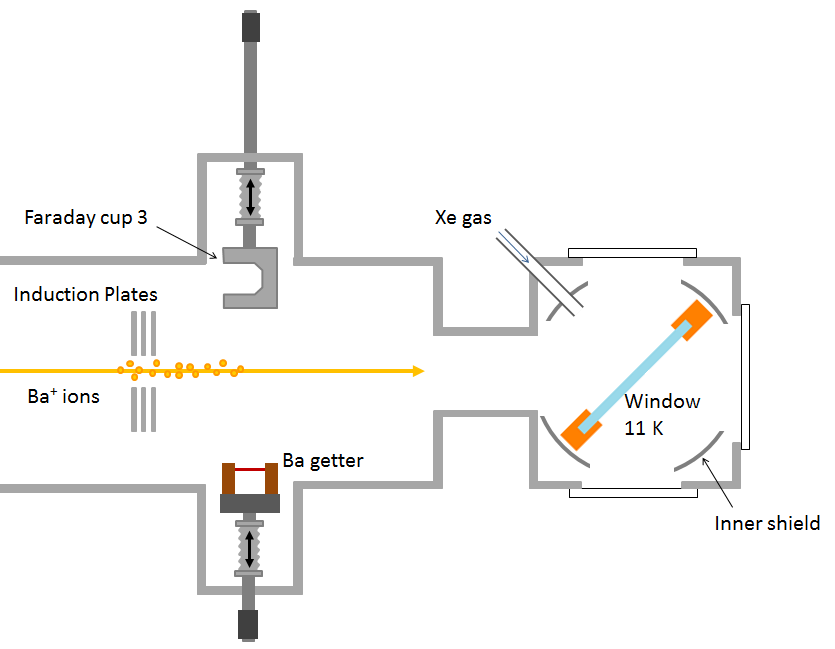
\includegraphics[width=.75\textwidth]{figures/window_etc_justBa.png}
                \caption{Apparatus near sapphire window, including Ba getter, Faraday cup 3, induction plates, and Xe gas inlet.}
\label{fig:endOfBeamBa}
\end{figure}

%\begin{figure} %[h]
%        \centering
%                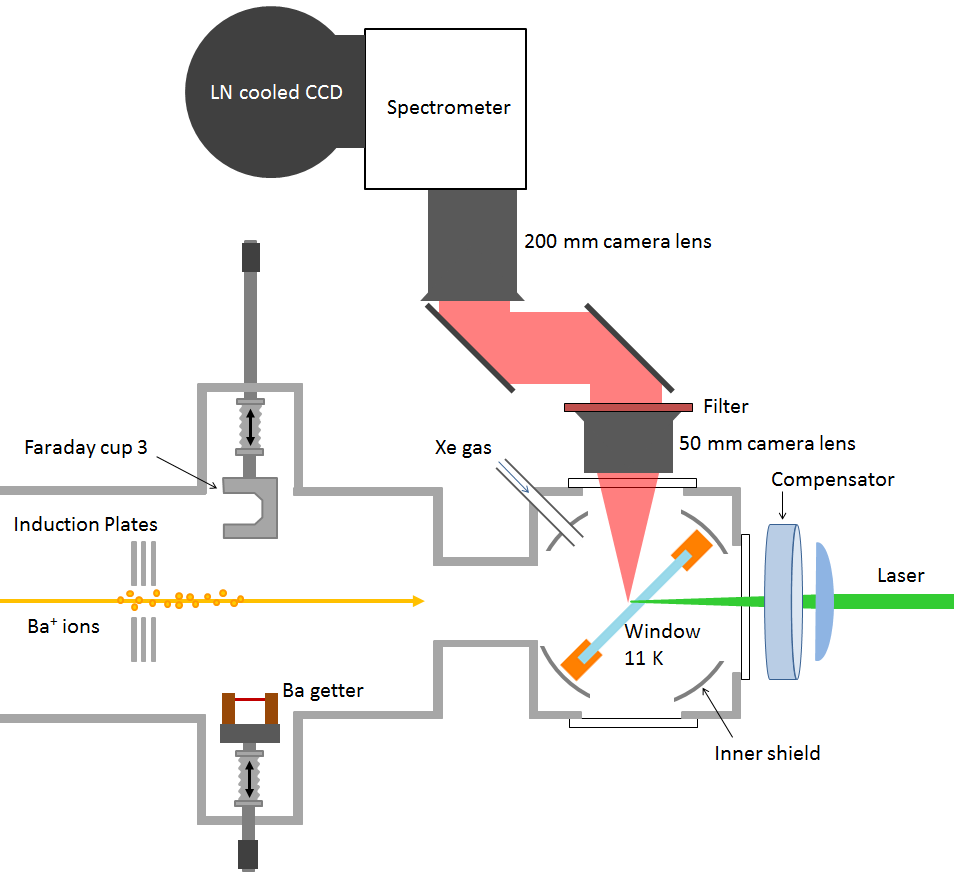
\includegraphics[width=.9\textwidth]{figures/window_etc.png}
%                \caption{Apparatus in spectroscopy region, including Ba getter, Faraday cup 3, induction plates, and optics for excitation, fluorescence collection, spectroscopy and detection.}
%\label{fig:endOfBeam}
%\end{figure}

\section{Sample Deposition}
\label{sec:deposition}

The Ba\textsuperscript{+}/Ba is co-deposited with ultra-pure Xe gas onto a cold sapphire window.  Sapphire has good thermal conductivity at low temperature and good optical transparency in the visible.  The window is held in a copper mount attached to a coldfinger and is tilted at 45$^{\circ}$ to allow access of the ion beam and Xe gas, as well as the excitation laser and collection optics.  To begin a deposit, Xe gas is flowed toward the window via a leak valve.  Cup 3 is then retracted and the ion beam is pulsed, depositing Ba\textsuperscript{+} ions into the SXe matrix as it grows.  Cup 3 is then replaced, and the Xe leak stopped.

\begin{figure} %[h]
        \centering
                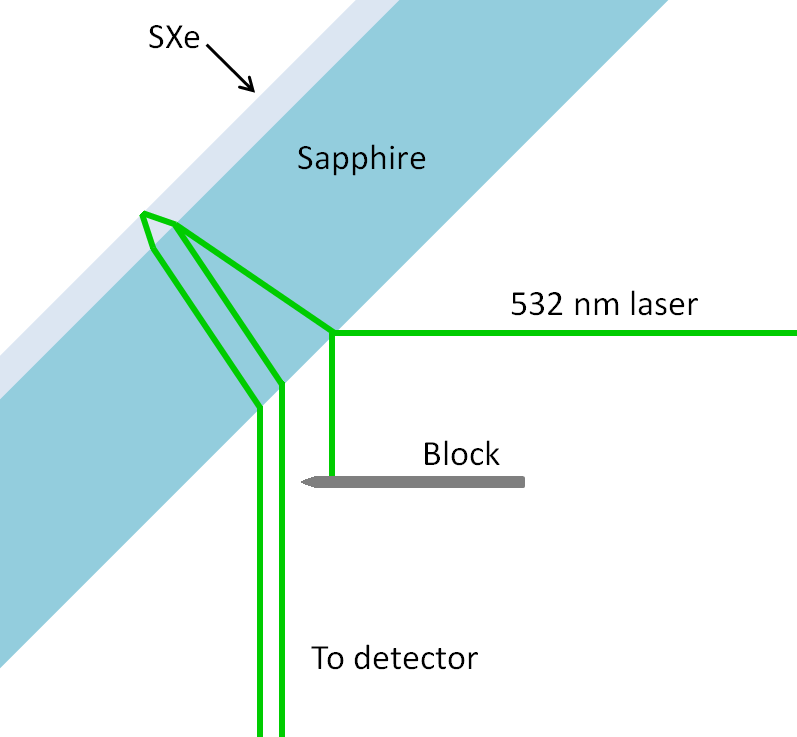
\includegraphics[width=.4\textwidth]{figures/fringe_setup.png}
                \caption{Setup for measuring SXe deposition rate by interference fringes.}
\label{fig:fringe_setup}
\end{figure}

\begin{figure} %[h]
        \centering
                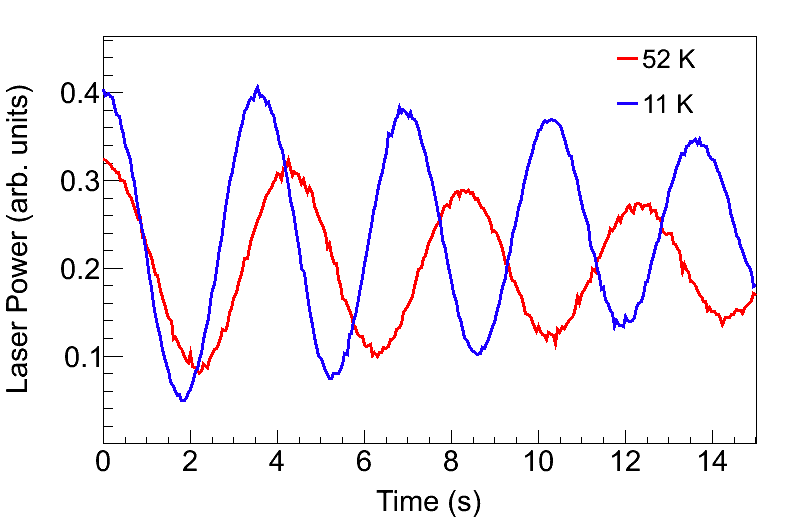
\includegraphics[width=.5\textwidth]{figures/fringes_52K_vs_11K.png}
                ~
                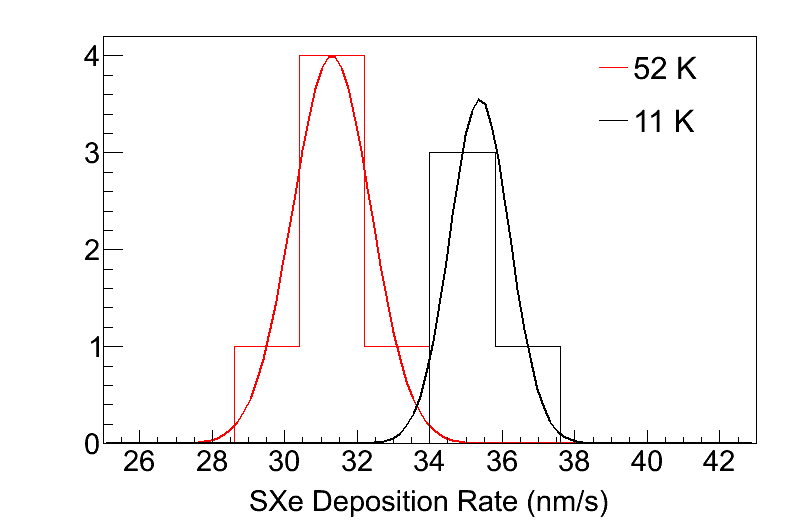
\includegraphics[width=.5\textwidth]{figures/fringes_52K_vs_11K_statistics.png}
                \caption{Interference fringes for the same Xe gas leak rate deposited on the sapphire window at 11~K and at 52~K.}
\label{fig:fringes_52K_vs_11K}
\end{figure}

SXe matrix deposition rate can be measured by interference fringes in a laser reflected against the front surface of the sapphire window, as shown in Fig. \ref{fig:fringe_setup}.  Fringes for SXe deposition at 52~K and 11~K are shown in Fig. \ref{fig:fringes_52K_vs_11K}(a) for the leak rate used in this work.  The refractive index of SXe has a negligible dependence on temperature between 50~ and 30~K \cite{SXeIndex}, so these can be compared directly.  A distribution of SXe deposition rate measurements from several deposits is shown in Fig. \ref{fig:fringes_52K_vs_11K}(b).  A somewhat lower rate is observed at 52~K, $31.3 \pm 0.44(\text{stat}) \pm 0.31(\text{sys})$~nm/s, vs. $35.4 \pm 0.41(\text{stat}) \pm 0.35(\text{sys})$~nm/s at 11~K.  Statistical errors are $\sigma / \sqrt{N}$ where $\sigma$ is the standard deviation of the Gaussian fits to the distributions in Fig. \ref{fig:fringes_52K_vs_11K}(b), and $N$ is the number of entries.  Systematic errors come from propagating an uncertainty on the angle between the laser and sapphire window of $\pm 2^{\circ}$.

\begin{figure} %[h]
        \centering
                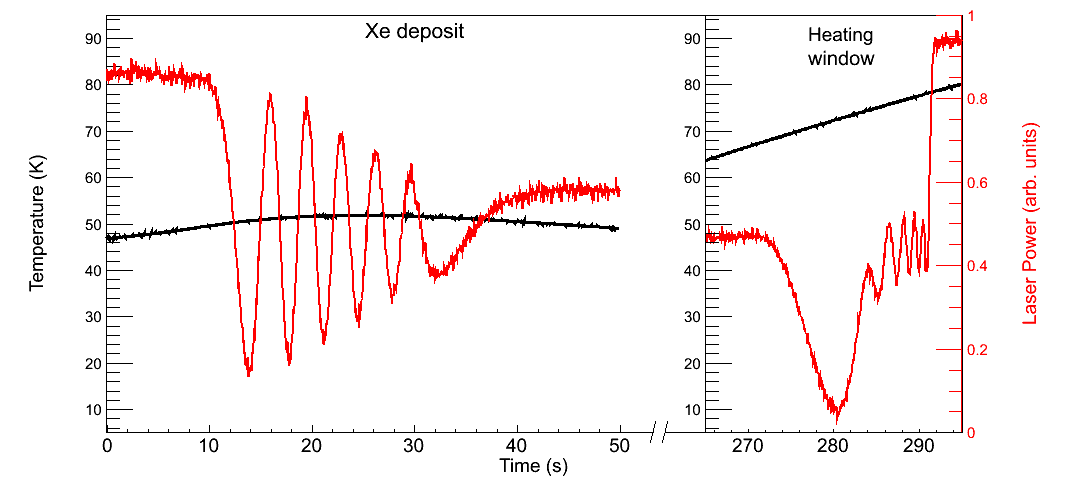
\includegraphics[width=.9\textwidth]{figures/fringes_dep_and_melt.png}
                \caption{(a) Interference fringes of a deposit at 52~K and of its subsequent evaporation when heating the sapphire window, and (b) distribution of SXe deposition rates calculated from fringe period of several measurements.}
\label{fig:fringes_melt_withDep}
\end{figure}

To evaporate a sample, the window is heated to 100~K.  Fringes appear during this process as well.  The full set of fringes for a deposit at 52~K and its evaporation when heated is shown in Fig. \ref{fig:fringes_melt_withDep}, along with the window temperature.  This shows that the SXe evaporates between 73~K and 78~K.  The same number of fringes appear in the deposit and the evaporation, indicating that the lower deposition rate at around 50~K is not due to simultaneous evaporation.  The variance in temperature during the deposit is due to the heater cycle.  Note that these Xe deposits were longer than for a typical deposit during a fluorescence experiment, in order to observe several fringes.

%quadrature errors: 0.54 for 52 K and 

\section{Laser Excitation}

\begin{figure} %[h]
        \centering
                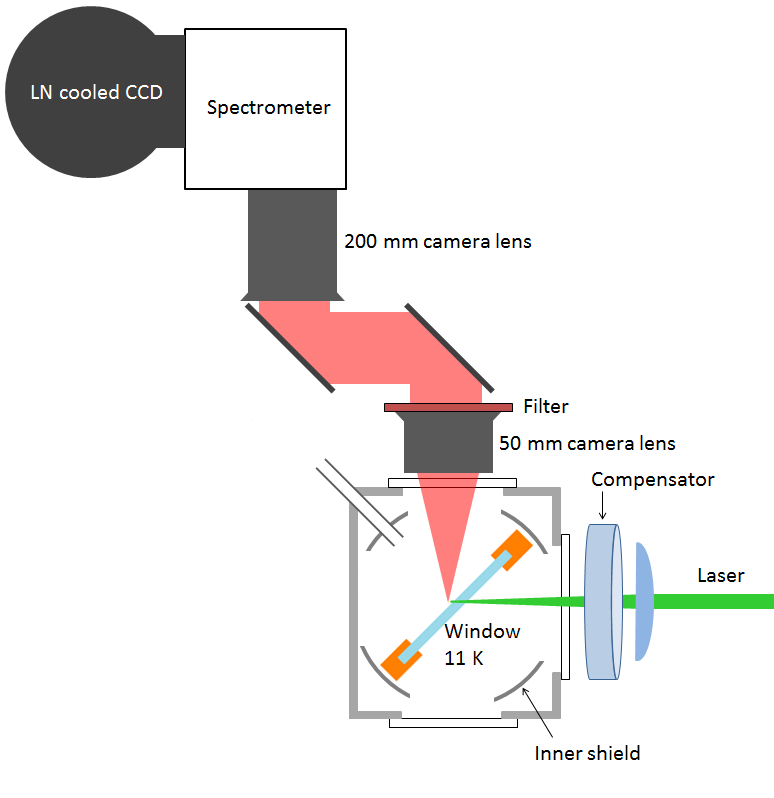
\includegraphics[width=.7\textwidth]{figures/window_etc_justOptics.png}
                \caption{Apparatus in spectroscopy region, including optics for excitation, fluorescence collection, spectroscopy and detection.}
\label{fig:endOfBeamOptics}
\end{figure}

Green to yellow laser excitation was done with a Coherent 599 dye laser, pumped by the 514-nm line of a Lexel 3500 Ar ion laser.  Rhodamine 110 (R110) dye was used for the 542 - 566~nm wavelength range, and Rhodamine 6G (R6G) for the 567 - 590~nm range.  Another Coherent 599 dye laser with Coumarin 480 (C480) dye was used for blue excitation, which was pumped by a Kr ion laser.  The Coherent 599 dye lasers were used with birefringent filters for wavelength tuning, but without etalons, since the broad absorption of Ba in SXe does not require single-mode laser excitation.

\begin{figure} %[h]
        \centering
                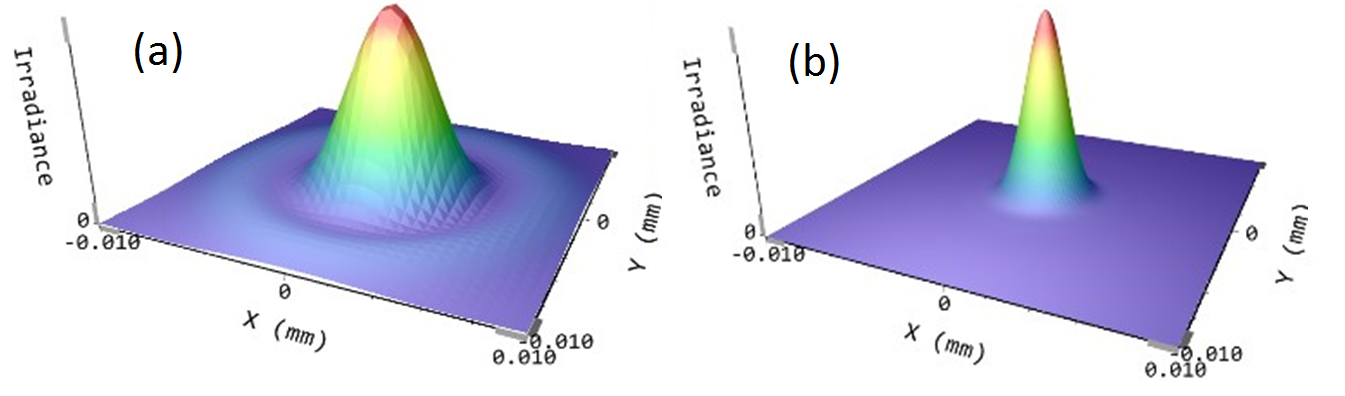
\includegraphics[width=.7\textwidth]{figures/DFairbank_aber.png}
                \caption{Calculated minimum laser spot size distributions, with wavelength 570~nm and unfocused waist w = 7~mm, for (a) bi-convex f = 7~cm lens, and (b) aspherical f = 7.9~cm lens.}
\label{fig:DFairbank}
\end{figure}

A lens focused the laser into the cryostat from the side, shown in Fig. \ref{fig:endOfBeamOptics}.  Initial work, spectroscopy (Chapter 4) and some imaging, was done using a bi-convex, which produced spherical aberration near the laser focus.  This effect does not affect the results in Chapter 4, where semi-focused beam waists of 100-1000~$/mu$m were used.  However, spherical aberrations caused the minimum beam waist to be about twice that of the diffraction limit.  To approach the diffraction limit in imaging small numbers (Chapter 5), a 7.9-cm focal length aspherical lens was used.  A comparison of the minimum spot sizes for these two lenses, calculated by David Fairbank at Thorlabs, is shown in Fig. \ref{fig:DFairbank}.

To correct for astigmatism introduced by the tilted sapphire window, compensating astigmatism was introduced by a fused silica optical flat of 1~cm thickness, placed after the lens, tilted on the y-axis (the laser is along the z-axis, and the sapphire window is tilted on the x-axis).  The proper angle for the compensator was determined to be about 10$^{\circ}$ from normal by a ray matrix calculation \cite{raymatrix}.  The effect of the SXe layer is negligible since its thickness is only about half a micron in a typical fluorescence experiment.  With the compensator, overlapping minimum spot sizes of 2.06~$\mu$m and 2.66~$\mu$m are calculated for x and y, respectively.  To observe the astigmatism and the effect of the compensator, the relative position of the x- and y-focus was observed by imaging 619-nm Ba fluorescence from a large deposit of Ba\textsuperscript{+} in SXe, with a varying laser focus.  For each z-position of the laser focusing lens, an image was taken, and a 2D Gaussian fit determined the x and y beam waists, w$_{\text{x}}$ and w$_{\text{y}}$.  Example fits to the 619-nm fluorescence for three laser focus positions, using the astigmatism compensator at 11$^{\circ}$, are shown in Fig. \ref{fig:astig}(a,b,c).  Gaussian fit values for w$_{\text{x}}$ and w$_{\text{y}}$ are plotted vs. laser focus position with (d) no compensator, and with the compensator at (e) 10$\pm 1^{\circ}$, (f) 13$\pm 1^{\circ}$, and (g) {\color{red}11}$\pm 1^{\circ}$.  With no compensator (d), the focal positions for x and y are measured to be about {\color{red}120}~$\mu$m apart, \emph{\color{gray}which is consistent with the calculated value of {\color{red}??}~$\mu$m from...}  10$\pm 1^{\circ}$ (e) and 13$\pm 1^{\circ}$ (f) can be seen to under- and over-shoot, respectively, the optimal angle, and {\color{red}11}$\pm 1^{\circ}$ (g), which was used in imaging experiments, is optimal, i.e. the x and y foci are consistent to within 50~$\mu$m.  \emph{\color{gray}A systematic uncertainty... on the beam size is then obtained ... leading to a focused laser spot of ?? $\pm$ ?? $\mu$m\textsuperscript{2}}

\begin{figure} %[H]
        \centering
                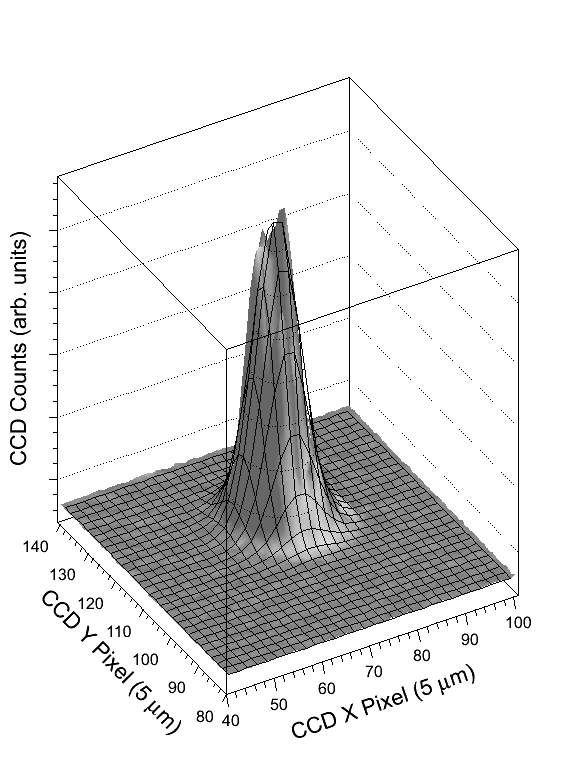
\includegraphics[width=.33\textwidth]{figures/astig_thesis_2Dgaus_run35.png}
                ~
                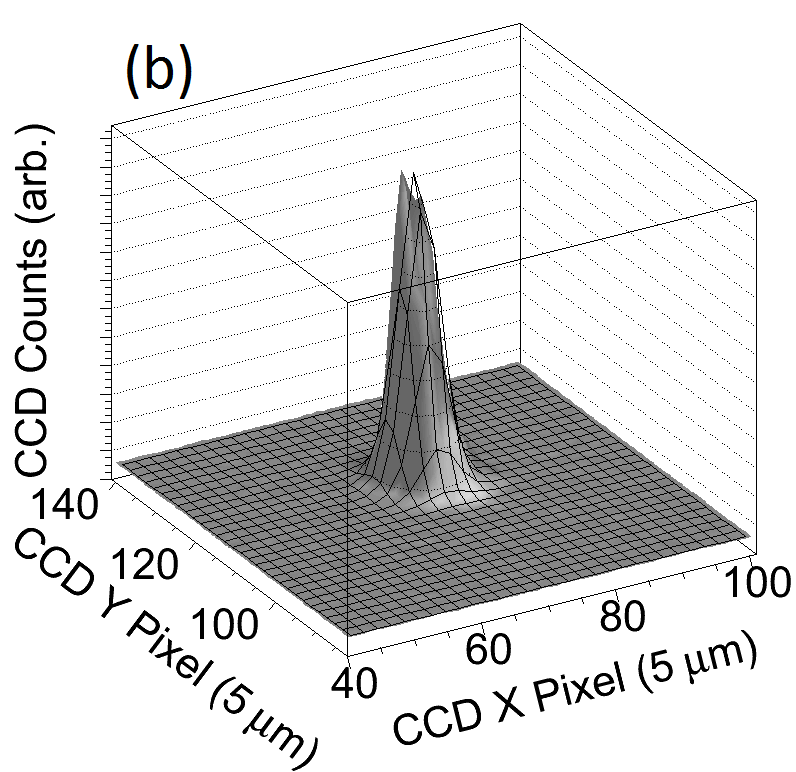
\includegraphics[width=.33\textwidth]{figures/astig_thesis_2Dgaus_run39.png}
                ~
                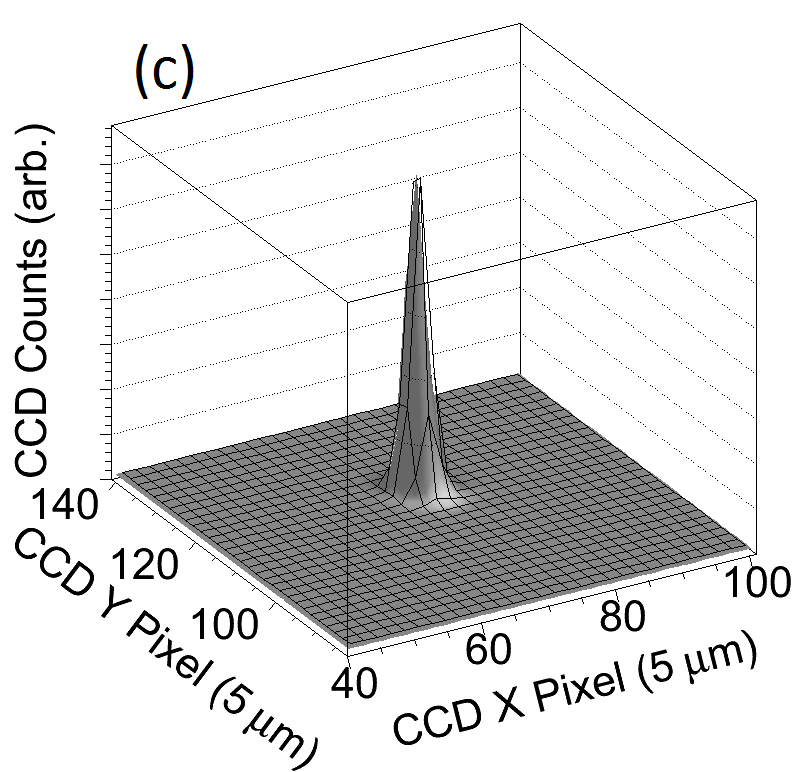
\includegraphics[width=.33\textwidth]{figures/astig_thesis_2Dgaus_run43.png}
                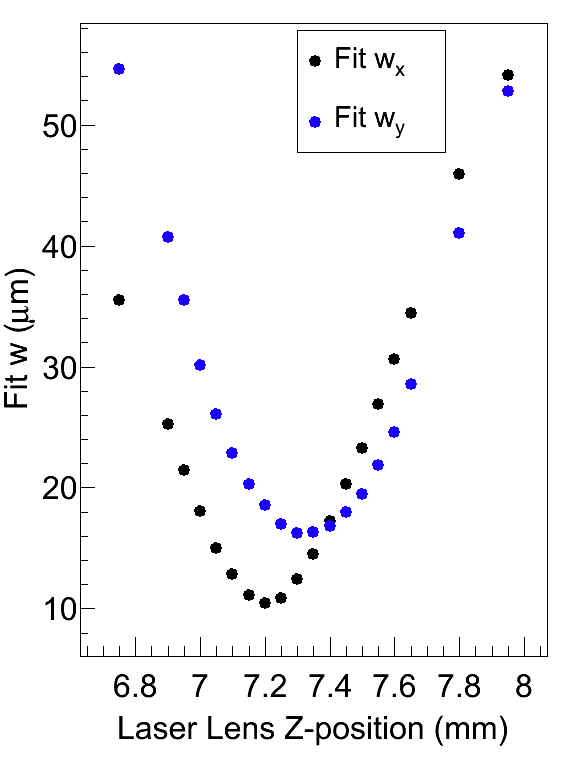
\includegraphics[width=.33\textwidth]{figures/astigcorr_curve_no-corr_806.png}
                ~
                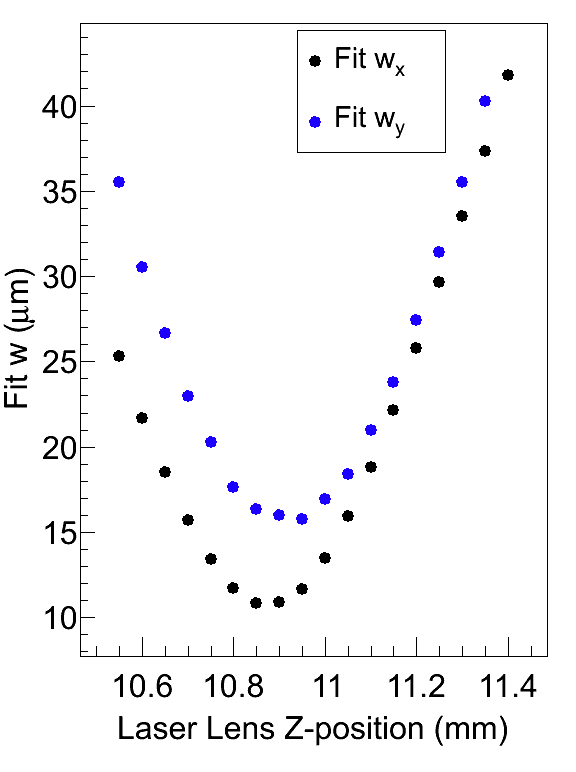
\includegraphics[width=.33\textwidth]{figures/astigcorr_curve_corr_10deg.png}
                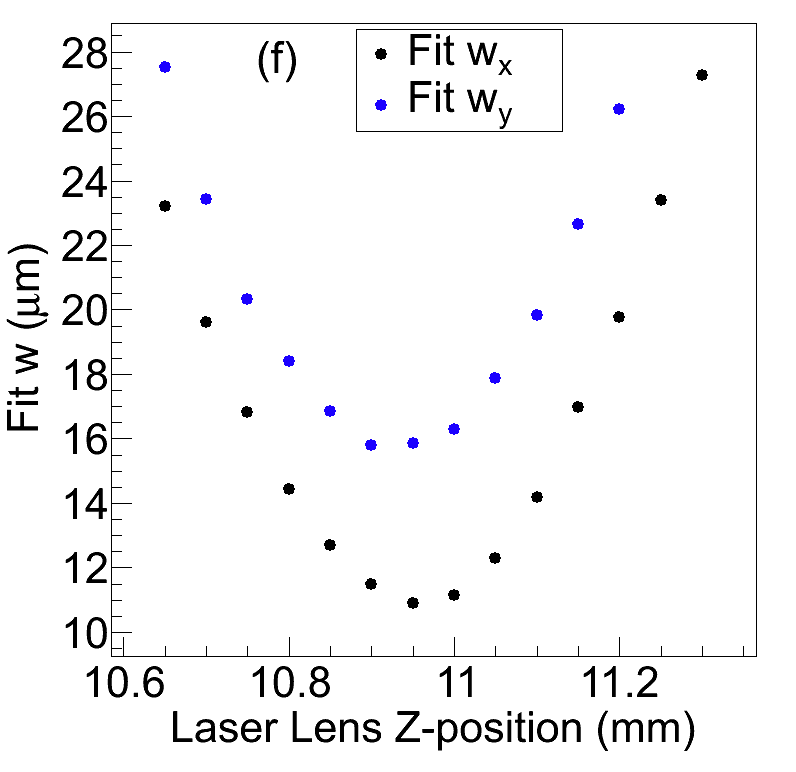
\includegraphics[width=.33\textwidth]{figures/astigcorr_curve_corr_13deg.png}
                ~
                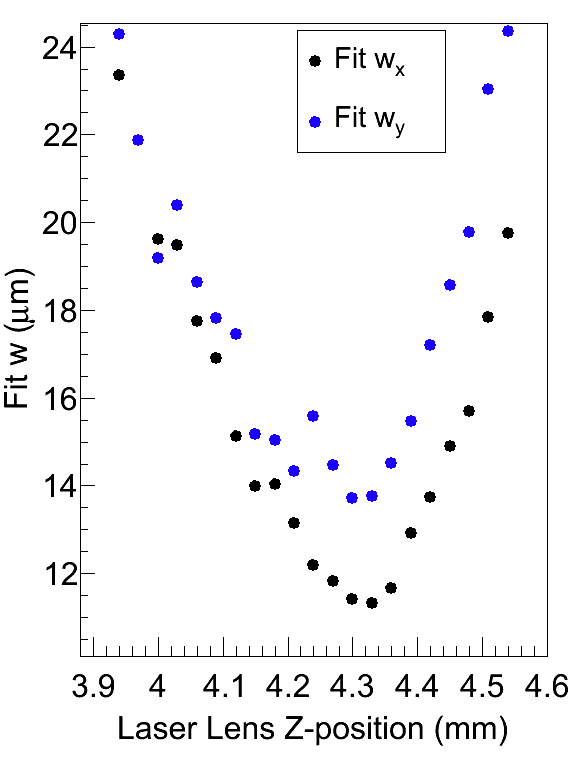
\includegraphics[width=.33\textwidth]{figures/astigcorr_curve_corr_9-16.png}
                \caption{Example 2D Gaussian fits (black grid lines) with varying laser focus (a,b,c) \emph{\color{gray}Needs larger text} .. \emph{\color{gray}make them squished more -- square}}
\label{fig:astig}
\end{figure}

%[waist measurements? -- apply calibration uncertainty to the good motor-stage ones]

%show measurements of astig. w/ and w/o compensator.?  8-7 prolly best so far

%Astigmatism in the laser itself was measured to be consistent with zero. (pg. 24 of Chris's book)
\section{Collection Optics}
\label{sec:collection}

Fluorescence was collected above the cryostat (Fig. \ref{fig:endOfBeamOptics}).  A 50~mm Nikon camera lens collimated the light, and a fluorescence filter sat on top of it.  A band-pass filter was used for imaging, and a Raman filter was used for spectroscopy.  The fluorescence then reflected off two steering mirrors, and was imaged by a 200~mm Nikon camera lens onto a Roper Scientific liquid-nitrogen-cooled CCD, with a magnification of 4.  The CCD has a quantum efficiency of 90\% in the visible, and in slow ADC mode, records one count per two photons collected.  At the set point of -100~$^{\circ}$C, dark counts are negligible.

The CCD has a removable Princeton Instruments imaging spectrometer.  With this attached, the 200~mm camera lens focuses the light onto an inlet slit, which is then imaged by the spectrometer onto the CCD after reflecting off a diffraction grating.  The 0-order reflection of the grating provides an image for alignment, and the grating can be tilted to distribute the 1\textsuperscript{st}-order reflection across the horizontal CCD pixels for doing spectroscopy.

When a 1" diameter filter is used, the imaging system has a solid angle collection of about 1.5\%.  Each additional component in the collection optics, listed in Table \ref{table:colleff}, contributes some loss, resulting in a total collection efficiency ($\epsilon_{c}$) of {\color{red}??} with the spectrometer, and {\color{red}??} without.  The spectrometer also limits the system to an f-number of 4, though this is not limiting in this setup.

\begin{table} [!htbp]
\caption{Factors contributing to optical collection efficiency.}
\label{table:colleff}
\begin{tabular}{l l l}
Component & Efficiency & \\
\hline
Cryostat Window & 0.99 & \\
Camera Lenses ($\times 2$) & {\color{red}??} & \\
Steering Mirrors ($\times 2$) & 0.95 & \\
CCD Quantum Efficiency & 0.90 & \\
Filter & 0.98 & \\
Counts per Photon (CCD) & 0.5 & $\epsilon_{c}\text{(w/o spectrom.)} = ${\color{red}??}\\
\hline
Spectrom. Mirrors ($\times 2$) & {\color{red}??} & \\
Diffraction Grating & 0.5 & $\epsilon_{c}\text{(w/ spectrom.)} = ${\color{red}??}\\
\end{tabular}
\end{table}

To limit laser exposure to only the time of CCD exposure, a laser shutter was linked to the camera exposure with a LabVIEW program.  This program also recorded laser power via a calibrated pickoff, as well as the temperature of the coldfinger near the sapphire window during observation.

\section{Vibrations and Effective Laser Region}

\begin{figure} %[H]
        \centering
                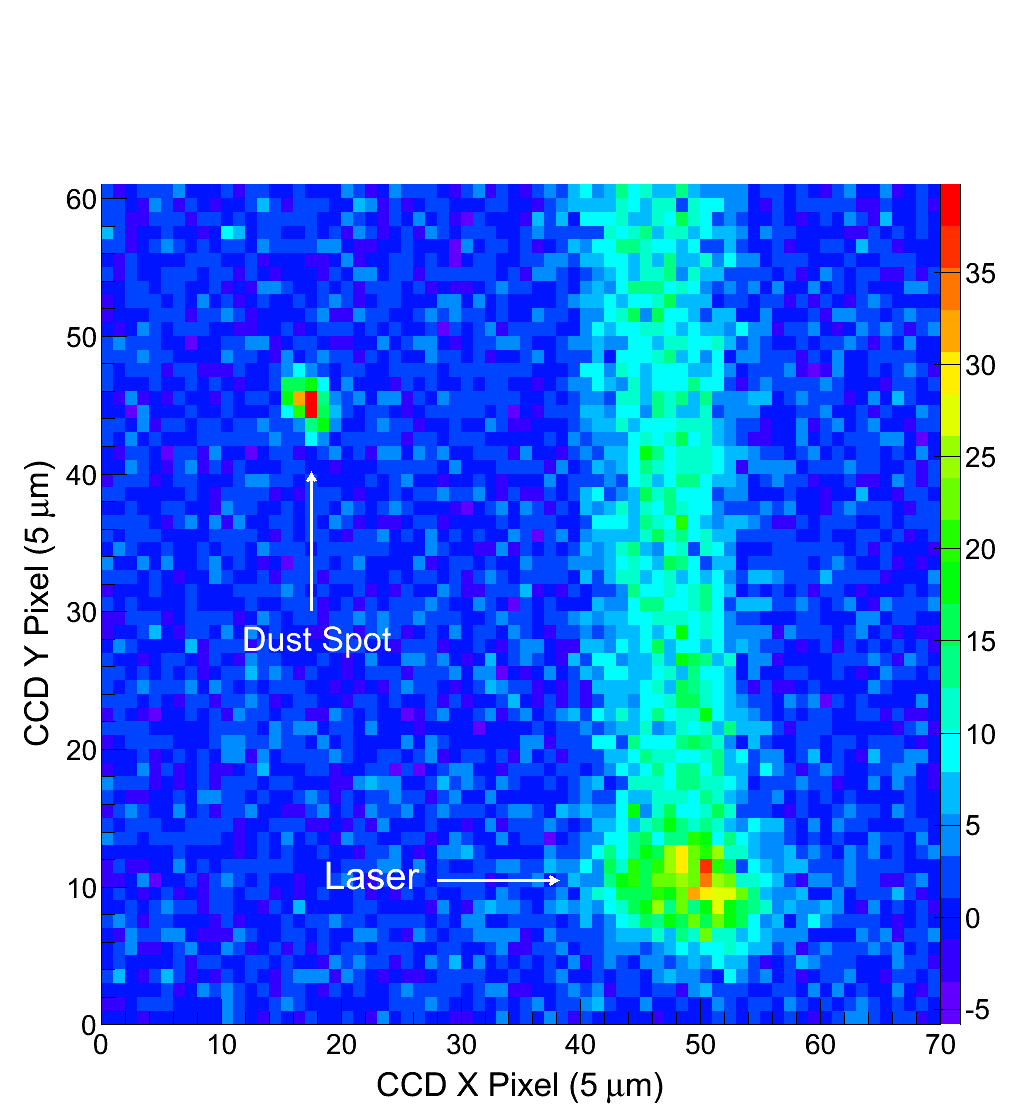
\includegraphics[width=.6\textwidth]{figures/image_dustspot.png}
                \caption{Example image of dust spot and laser during observation of cryostat vibrations.}
\label{fig:dustspot}
\end{figure}

Relative vibrations between the laser and sapphire window affect the number of Ba atoms exposed, increasing the effective laser spot size.  This was studied by observing the position of a ``dust spot" (a highly scattering feature on the sapphire window) relative to the position of the laser in an image on time scales down to 50~ms.  An example of an image from this experiment is shown in Fig. \ref{fig:dustspot}.  The 570-nm dye laser was somewhat de-focused, and the dust spot was illuminated by a de-focused 657~nm diode laser. For each frame, 2D Gaussian functions were fit to locate the center of the laser spot and the dust spot in order to measure their relative position.  The fit for the laser spot was restricted in y so that it was not affected by the bulk sapphire fluorescence path.  The distances in x and y between the dust spot and laser are plotted for each 50-ms snapshot in Fig. \ref{fig:cryovibe2D}(a).  The distribution shows a correlation between x and y.  To calculate an effective laser spot size due to this vibration, each difference (x,y) between laser and dust spot was used as the center of a 2D Gaussian, each with w$_{x} = 2.06~\mu$m and w$_{y} = 2.66~\mu$m to represent the laser spot.  Such Gaussian functions were summed for all points to produce a distribution of summed laser exposure, shown in Fig. \ref{fig:cryovibe2D}(b).  The total area enclosed by a 1/e contour then represents the effective area.  Since x and y movement are correlated, and since the movement is sinusoidal, the effective area is only about {\color{red}2$\times$} \emph{\color{gray}make an ``if greater than or equal to 1/e" thing for bins} the real laser spot size, and the effective laser region is {\color{red}17.8~$\mu$m$^{2}$}.

%The difference between dust spot and laser positions is plotted in {\color{red}Fig. [fig vibe vs. time with sine fit]} for both x and y.  Each exposure in this plot is 50~ms, though readout time and camera shutter compensation time result in x~s between frames.  The best fit of a sine function results in a vibration frequency of x~Hz.  This is consistent with the audible frequency of the cryostat He pump.
%...could do this for rotated

\begin{figure} %[H]
        \centering
                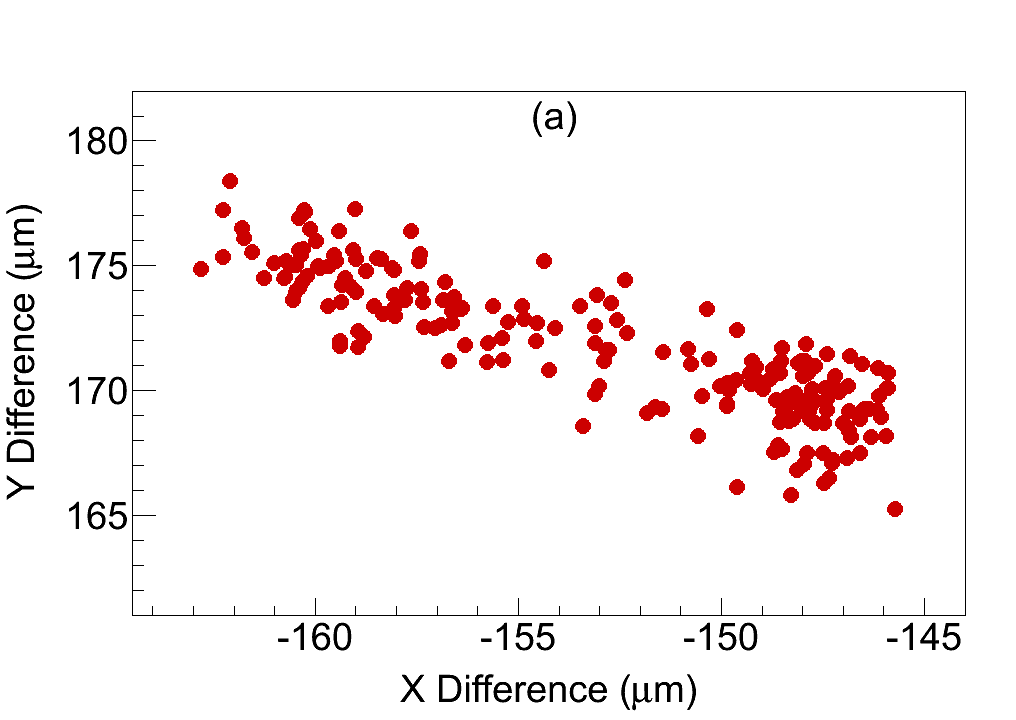
\includegraphics[width=.5\textwidth]{figures/cryovibes_a.png}
                ~
                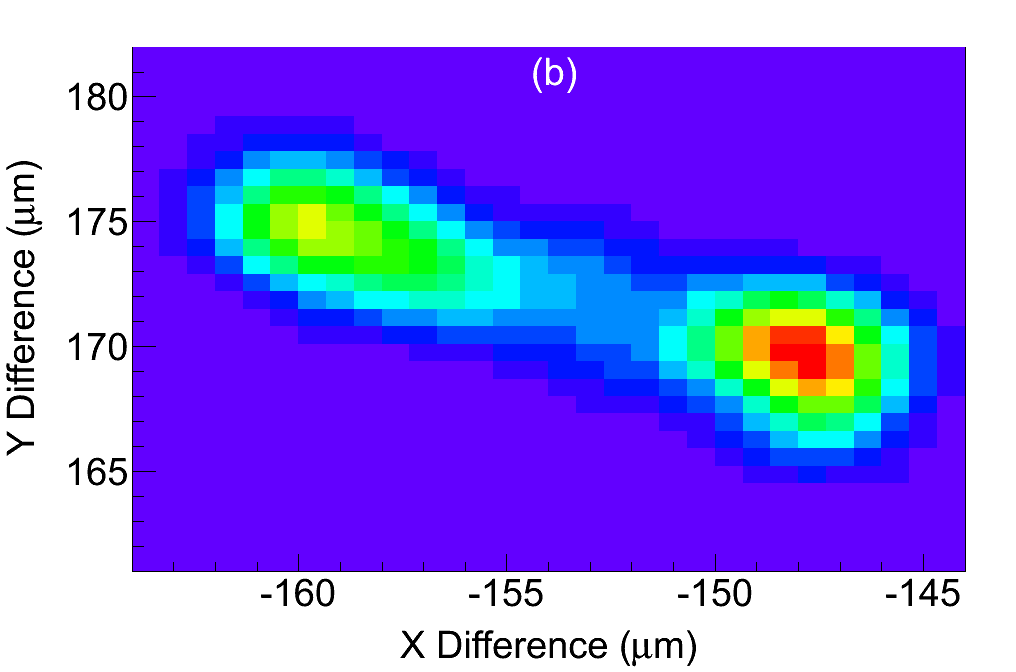
\includegraphics[width=.5\textwidth]{figures/cryovibes_b.png}
                \caption{Cryostat vibration measurements based on relative position of dust spot vs. laser on sapphire window in 50-ms snapshots (a), with 2D Gaussians overlain on each point to represent total laser exposure vs. position (b).}
\label{fig:cryovibe2D}
\end{figure}

The aforementioned is the most concerning vibration to understand.  Vibration of the laser itself is included in that study.  Vibration of the collection optics will affect the imaging resolution, but not the number of atoms being observed.  These vibrations were minimized by stable mounts.

\section{Laser Scanning}
\label{sec:laserscanning}

In order to obtain images of separated single atoms, the laser focusing lens is attached to motorized Newport translation stages which scan the laser position by scanning the lens in x and y, shown in Fig. \ref{fig:laserStages}.  These stages sit atop a manual z-translation stage for laser focusing.  An extension of the aforementioned LabVIEW program coordinates movement of these stages such that x or y position is stepped in between CCD frames, and each frame then corresponds to a position in a laser scan grid.

\emph{\color{gray}Show data on steps and reproducibility -- say this isn;t good and new stages will be used later.}

\begin{figure} %[h]
        \centering
                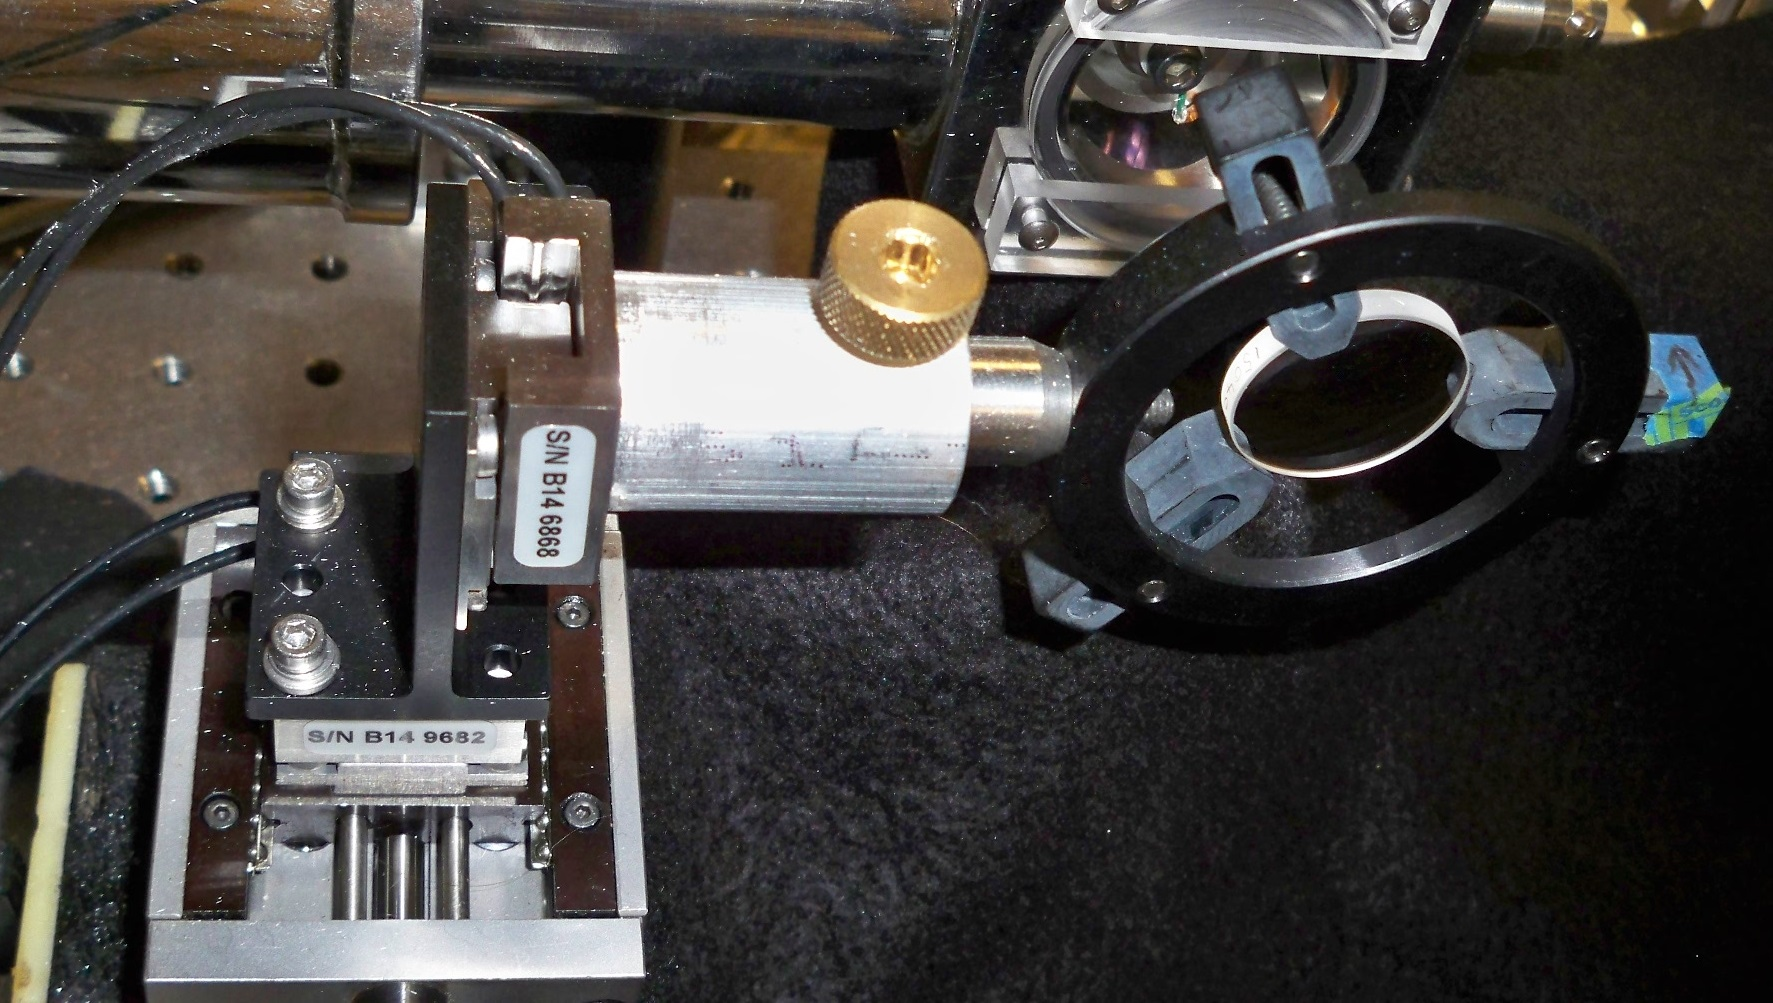
\includegraphics[width=.5\textwidth]{figures/stages_2.JPG}
                \caption{Asphere laser focusing lens mounted to motorized Newport translation stages for laser scanning.}
\label{fig:laserStages}
\end{figure}
